\section{Distributed self-adjusting systems}
\label{sec:architecture}

Next we show a general distributed systems architecture, which, as we show theoretically and empirically later, produces faster-than-linear scaling in several disparate problem domains. Our main observation is that, whenever genuinely observed, superlinear scaling assumes two critical components: a policy to dispatch jobs to workers in a way to increase the locality of reference in the per-worker input streams, plus an algorithm that can adaptively exploit the structure in the input to process it more efficiently. Our architecture is purely a software technique in that it does not require the addition of new cache space to a system. Nonetheless, it contains distributed caching as a special case and hence automatically takes advantage of additional fast memory, if available.

\subsection{Locality-boosting load balancing}
\label{sec:lb-lb}

The first crucial component in our architecture is a locality-boosting load balancer.  In this context, load balancing refers to the distribution of computational work or incoming network traffic across multiple parallel workers (servers, processors, or nodes). A good load balancing strategy ensures optimal resource utilization, minimizes response time, avoids overloading any single resource, and, as we argue below, improves the locality in the input presented to the workers. 

In the context of this paper, \emph{locality of reference} is the property of a sequence of inputs that subsequent items are statistically dependent on each other. Such structure in the input can then be readily exploited by the proper algorithm \cite{SleatorT85Splay, BentleyCL93, HesterH85, HesterH85, BentleySTW86, Avin0020, ParkM12} or a runtime optimization framework \cite{276946,246322,10.1145/3503222.3507769,procieee_2019} to improve the performance of the code that processes it. A request set with minimal locality is uniformly distributed on the entire domain of possible inputs and hence unpredictable, while one with maximal locality contains only a single item, i.e., maximally predictable. A \emph{locality-boosting load balancing} policy is then a request dispatching strategy that can statistically or deterministically improve the locality of reference experienced by the worker threads, \emph{turning an unpredictable system input into multiple streams of predictable inputs to be processed by the workers} (see Fig.~\ref{fig:locality-boosting-lb}).

\begin{figure}
  \centering
  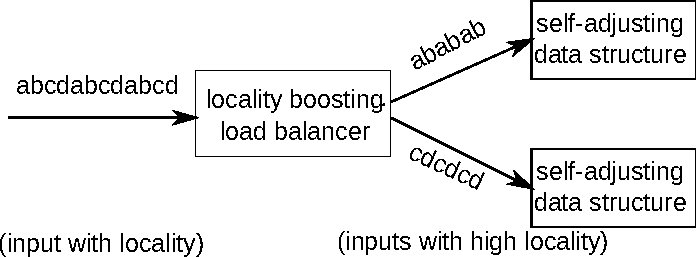
\includegraphics[width=.85\linewidth]{fig/schema.pdf}
  \caption{A locality boosting load balancer partitions the input sequence of a given locality into subsequences with higher locality. Self-adjusting data structures perform better on inputs with higher locality.}
  \label{fig:locality-boosting-lb}
\end{figure}

We distinguish two types of locality in this context. \emph{Spatial locality} means that the distribution of requested items on the entire input domain is statistically biased towards a particular subset of the items. One way to ensure this in the load balancer is to \emph{partition} the input domain into disjunct subsets, so that worker's input distributions are concentrated on a smaller set of inputs. For instance, the hash-based load balancer we used previously to show superlinear scaling with distributed caching is such a partitioning load balancer. In contrast, a round robin or a uniform random load balancer will export its own spatial input locality unchanged to the workers. A related concept is \emph{temporal locality}, which refers to the reuse of specific items in the input within a relatively small time duration. One way to boost temporal locality is to reorder items within a time window: e.g., Reframer applies controlled delays to particular packets in a packet batch to boost temporal locality and, thereby, enable more efficient processing \cite{276946,246322}.

\subsection{Self-adjusting algorithms}
\label{sec:sa-alg}

The second critical enabler for superlinear scaling in our architecture is \emph{self-adjusting algorithms}. Self-adjustment is a general term referring to the property of a dynamic data structure to \emph{automatically reorganize itself based on the sequence of operations it receives}, in order to optimize performance for future operations on frequently accessed or manipulated elements. Internal data reorganization always introduces extra complexity and overhead compared to a static data structure. Therefore, self adjustment can improve performance only if the input processed by the algorithm exhibits a certain amount of spatial or temporal locality.

Next we review the most prominent self-adjusting data structures (but see also \cite{BoseDL08, Avin0020, ParkM12}).

% For further examples, see self-adjusting skip lists~\cite{BoseDL08}, push-down trees~\cite{Avin0020}, or geometric data storages \cite{ParkM12}.

\noindent%
\textbf{Caches.} %
As the simplest but most universal self-adjusting data structure, caches can serve frequently accessed items fast by storing them in a  software or a hardware fast memory. This is typically much faster than if we had to run the request through the full processing pipeline or the slow backing store. Thus, caches have that almost magical capability of self-adaptation, without us having to engineer any prior knowledge of the input into the cache mechanism apart from a promise that it has nontrivial locality. When the promise is true, caches are an inexpensive way to improve throughput and response time. When there is no locality in the input, however, caches usually just add extra latency and overhead.
%
Note that caches do not necessarily have to come in the form of hardware memory: a fast key-value store is a candidate cache for a slow database \cite{10.5555/1012889.1012894}, a kernel fast-path flow cache is a useful way to speed up a slow user-space software switch \cite{188960}, etc.

% However, caches also come with additional complexity and overhead: cache entries have to be created for storing recently accessed data, invalidated when the backing data changes, evicted when the cache is full, and synchronized to consistently represent data that may be present in multiple caches. % Hardware implementations are appealing from this aspect by hiding the extra complexity behind a fast on-chip implementation.

% The performance of a cache is determined by the cache hit rate $\delta$, defined as the ratio of operations served from fast memory to those served on the slow path, and $\rho$, the penalty of a cache miss. In general, for a common LFU or LRU cache the higher the locality in the input and the bigger the cache compared to the input domain, the higher the cache hit rate and the lower the response time. When there is no locality in the input, caches usually just add extra latency and overhead.

\noindent%
\textbf{List lookup.} %
One of the most widely used self-adjusting data structures is the \emph{move-to-front list}. Suppose we wish to store a list of $m$ items in a way so that reordering, insertion and deletion are fast, while lookup is also reasonably efficient. A straightforward choice is a static linked list. Here, the cost of accessing an item at position $i$ is exactly $i$. Then, any linked list can easily be upgraded to a self-adjusting list using the move-to-front (MTF) heuristics: after accessing an item it is moved to the front, which improves lookup time for future requests of the same item at minimal cost (see Fig.~\ref{fig:mtf-example}). The MTF heuristics comes with appealing theoretical properties, namely that unconditionally moving the accessed item to the front of the list is close to the best one could achieve, even if one knew all future requests \cite{SleatorT85}. MTF can handle both spatial and temporal locality. However, for uniformly distributed input MTF lists usually add nontrivial overhead compared to static lists due to the frequent and useless relinking of the list.

\begin{figure}
  \centering
  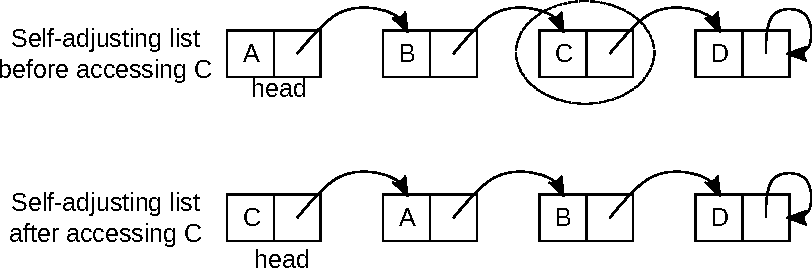
\includegraphics[width=.85\linewidth]{fig/mtf.pdf}
  \caption{A self-adjusting list containing nodes A,B,C and D serves the request to C and moves C to the front of the list to speed up future accesses to C.}
  \label{fig:mtf-example}
\end{figure}

Classic applications of MTF lists are information retrieval systems, compression~\cite{BentleySTW86}, etc. In general, any use case is a potential candidate application for MTF where the task is to match a request against a list of complex rules that do not lend themselves readily to be arranged into a fast lookup structure (e.g., a search tree), like inference in explainable rule-based AI % and expert systems
\cite{dovsilovic2018explainable}, rule matching in OpenFlow and P4 reference software switches \cite{openflow}, packet classification in networking (see later), etc.  We note that caching is a subset of list lookup, in that every algorithm for list reorganization gives rise to a different cache management algorithm \cite{SleatorT85}.  

\noindent%
\textbf{Search trees.} %
A search tree is an efficient tree data structure for locating specific keys from within an ordered set. A \emph{splay tree} is a self-adjusting version of a static search tree, in that it can dynamically reorganize itself by moving popular items closer to the root of tree and less frequently accessed elements to the bottom, while keeping the tree relatively well-balanced \cite{SleatorT85Splay, BoseDL08, Avin0020}. Since access time in a search tree is determined by the depth at which the requested item is to be found, splay trees can improve future access to the same or similar items when the input exhibits temporal or spatial locality (see Fig.~\ref{fig:bst_root_3}).  Note that a red-black tree, an AVL tree or any similar self-balancing tree is not self-adjusting, in that it can rearrange only with respect to the items \emph{stored} in it but not with respect to the queries \emph{posed} to it.

\begin{figure}
 \centering
 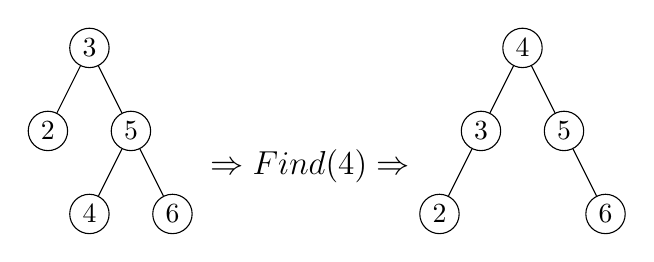
\begin{tikzpicture}[level distance=30pt,
   level 1/.style={sibling distance=30pt},
   level 2/.style={sibling distance=30pt},
   level 3/.style={sibling distance=30pt}]
   % Left
   \node[circle,draw,minimum size=0.5cm,inner sep=1pt] (3a) {3}
   child {node[circle,draw,minimum size=0.5cm,inner sep=1pt] (2a) {2}}
   child {node[circle,draw,minimum size=0.5cm,inner sep=1pt] (5a) {5}
     child {node[circle,draw,minimum size=0.5cm,inner sep=1pt] (4a) {4}}
     child {node[circle,draw,minimum size=0.5cm,inner sep=1pt] (6a) {6}}
   };
   % Right
   \node[circle,draw, minimum size=0.5cm, inner sep=1pt] (4b) at (5.5,0) {4}
   child {node[circle,draw,minimum size=0.5cm,inner sep=1pt] (3b) {3}
     child {node[circle,draw,minimum size=0.5cm,inner sep=1pt] (2b) {2}}
     child[missing] {}
   }
   child {node[circle,draw,minimum size=0.5cm,inner sep=1pt] (5b) {5}
     child[missing] {}
     child {node[circle,draw,minimum size=0.5cm,inner sep=1pt] (6b) {6}}
   };
   % Arrow
   \node (draw=none) at (2.8,-1.5) [font=\large]{$\Rightarrow{Find(4)}\Rightarrow$};
 \end{tikzpicture}
 \caption{Splay-tree with elements 2, 3, 4, 5, 6. After accessing node 4 it is moved to the root that makes a subsequent lookup to it faster, while the tree is kept almost perfectly balanced.}
 \label{fig:bst_root_3}
\end{figure}

\begin{figure*}[t]
  % \begin{tabularx}{\textwidth}{D *{2}{s}}
  \begin{tabular}{m{.3\textwidth} m{.31\textwidth} m{.31\textwidth}}
  % \begin{tabular}{ccc}
    \hspace{28pt}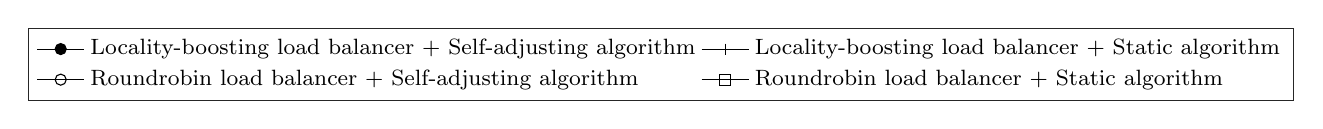
\begin{tikzpicture} 
  \begin{axis}[%
    height=45pt,
    hide axis,
    xmin=10,
    xmax=50,
    ymin=0,
    ymax=0.4,
    legend style={
      draw=white!15!black,
      legend cell align=left,
      legend columns=2,
      font=\footnotesize}
    ]
    \addlegendimage{black,mark=*}
    \addlegendentry{Locality-boosting load balancer + Self-adjusting algorithm}
    \addlegendimage{black,mark=+}
    \addlegendentry{Locality-boosting load balancer + Static algorithm}
    \addlegendimage{black,mark=o}
    \addlegendentry{Roundrobin load balancer + Self-adjusting algorithm}
    \addlegendimage{black,mark=square}
    \addlegendentry{Roundrobin load balancer + Static algorithm}
  \end{axis}
\end{tikzpicture}

%%% Local Variables:
%%% mode: latex
%%% TeX-master: "../distributed_mrf"
%%% End:
\\
    \multirow{-6.4}{*}{\subcaptionbox{List lookup/uniform input\label{fig:multicore-list-uniform}}{\begin{small}
  \begin{tikzpicture}
    \begin{axis}[
      width=165pt,
      height=322pt,
      xlabel={number of CPU cores},
      x label style={at={(0.5,0.01)}},      
      ylabel={Speedup},
      y label style={at={(0.05,0.5)}},      
      xmin=1,
      xmax=48,
      xtick={1,12,24,36,48},
      ymin=0,
      ymax=3300,
      legend style = {
        anchor = north west,
        at = {(0.01, 1.01)},
        font=\tiny,
        % draw = none,
      },
      % scaled y ticks=false
      % no markers
      ]
      % use TeX as calculator:
      \addplot[black,mark=*] table[x=thread,y=speedup,] {fig/list/uniform-100k/multicore_mtf_modulo_uniform.txt};
      % \addlegendentry{Move-to-front/Local LB}
      \addplot[black,mark=+] table[x=thread,y=speedup,each nth point={3}] {fig/list/uniform-100k/multicore_linkedlist_modulo_uniform.txt};
      % \addlegendentry{Linked-list/Local LB}
      \addplot[black,mark=o] table[x=thread,y=speedup,each nth point={3}] {fig/list/uniform-100k/multicore_mtf_roundrobin_uniform.txt};
      % \addlegendentry{Move-to-front/Non-local LB}
      \addplot[black,mark=square] table[x=thread,y=speedup,each nth point={3}] {fig/list/uniform-100k/multicore_linkedlist_roundrobin_uniform.txt};
      % \addlegendentry{Linked-list/Non-local LB}
    \end{axis}
  \end{tikzpicture}
\end{small}

%%% Local Variables:
%%% mode: latex
%%% TeX-master: "../../../distributed_mrf"
%%% End:
}}%
    & \hspace{18pt}\subcaptionbox{List lookup/Zipf input\label{fig:multicore-list-zipf}}{\begin{small}
  \begin{tikzpicture}
    \begin{axis}[
      width=165pt,
      height=322pt,
      xlabel={number of CPU cores},
      x label style={at={(0.5,0.01)}},      
      ylabel={Speedup},
      y label style={at={(0.05,0.5)}},      
      xmin=1,
      xmax=48,
      xtick={1,12,24,36,48},
      ymin=0,
      ymax=3300,
      legend style = {
        anchor = north west,
        at = {(0.01, 1.01)},
        font=\tiny,
        % draw = none,
      },
      % scaled y ticks=false
      % no markers
      ]
      % use TeX as calculator:
      \addplot[black,mark=*] table[x=thread,y=speedup,] {fig/list/uniform-100k/multicore_mtf_modulo_uniform.txt};
      % \addlegendentry{Move-to-front/Local LB}
      \addplot[black,mark=+] table[x=thread,y=speedup,each nth point={3}] {fig/list/uniform-100k/multicore_linkedlist_modulo_uniform.txt};
      % \addlegendentry{Linked-list/Local LB}
      \addplot[black,mark=o] table[x=thread,y=speedup,each nth point={3}] {fig/list/uniform-100k/multicore_mtf_roundrobin_uniform.txt};
      % \addlegendentry{Move-to-front/Non-local LB}
      \addplot[black,mark=square] table[x=thread,y=speedup,each nth point={3}] {fig/list/uniform-100k/multicore_linkedlist_roundrobin_uniform.txt};
      % \addlegendentry{Linked-list/Non-local LB}
    \end{axis}
  \end{tikzpicture}
\end{small}

%%% Local Variables:
%%% mode: latex
%%% TeX-master: "../../../distributed_mrf"
%%% End:
}
    & \hspace{8pt}\subcaptionbox{List lookup/uniform/single-core\label{fig:singlecore-list-uniform}}{\begin{small}
  \begin{tikzpicture}
    \begin{axis}[
      width=250pt,
      height=170pt,
      xlabel={\#thread},
      ylabel={Goodput [million req/sec]},
      xlabel near ticks,
      ylabel near ticks,
      xmin=1,
      xmax=26,
      ymin=0,
      % ymax=10,
      legend style = {
        anchor = north west,
        at = {(0.01, 1.01)},
        font=\scriptsize,
        % draw = none,
      },
      % no markers
      ]
      \addplot[black,mark=*] table[
      x=thread,
      y expr=\thisrowno{4}/1000000
      ]{fig/list/uniform-10/singlecore_mtf_modulo_uniform.txt};
      \addlegendentry{MTF w/ hash-based lb}
      \addplot[black,mark=+] table[
      x=thread,
      y expr=\thisrowno{4}/1000000
      ]{fig/list/uniform-10/singlecore_linkedlist_modulo_uniform.txt};
      \addlegendentry{Static list w/ hash-based lb}
      \addplot[black,mark=o] table[
      x=thread,
      y expr=\thisrowno{4}/1000000
      ]{fig/list/uniform-10/singlecore_mtf_roundrobin_uniform.txt};
      \addlegendentry{MTF w/ round robin lb}
      \addplot[black,mark=square] table[
      x=thread,
      y expr=\thisrowno{4}/1000000
      ]{fig/list/uniform-10/singlecore_linkedlist_roundrobin_uniform.txt};
      \addlegendentry{Static list w/ round robin lb}
    \end{axis}
  \end{tikzpicture}
\end{small}

%%% Local Variables:
%%% mode: latex
%%% TeX-master: "../../../hotnets22"
%%% End:
}
    \\
    & \hspace{18pt}\subcaptionbox{Cache lookup/uniform input\label{fig:multicore-cache-uniform}}{\pgfplotsset{
  RatePlot/.style = {
    tick pos = left,
    xtick align=outside,
    ytick align=outside,
    xlabel near ticks,
    ylabel near ticks,
    width=.4\textwidth,
    height=.3\textwidth,
    legend pos = north west,
    legend cell align=left,
    ylabel = {Throughput [Mpps]},
    xlabel = {number of CPU cores},
    xmin=1, xmax=32,
    ymin=0,
  },
  SpeedupPlot/.style = {
    RatePlot,
    ylabel={Speedup},
  },
  ClassBenchGroupPlot/.style = {
    group/group size = 1 by 2,
    group/horizontal sep = 0pt,
    group/vertical sep = 28pt,
  },
  ClassBenchRatePlot/.style = {
    RatePlot
  },
  ClassBenchSpeedupPlot/.style = {
    SpeedupPlot,
  }
}

%%% Local Variables:
%%% mode: latex
%%% TeX-master: "../distributed_mrf.tex"
%%% End:

%
\begin{small}
  % \tikzmath
  % {
  %   function est(\x)
  %   {
  %     if (\x < 10) then
  %     {
  %       return 0.1+0.9*(0.1*\x +(1-0.1*\x)*10)/\x;
  %     } else {
  %       return 0.1 + 0.9//\x;
  %     };
  %   };
  %   \a = est(4);
  %   \b = est(14);
  % }
  \begin{tikzpicture}
    \begin{axis}[
      width=165pt,
      height=120pt,
      xlabel={\#CPU cores},
      x label style={at={(0.5,0.04)}},
      ylabel={Speedup},
      % xlabel near ticks,
      % ylabel near ticks,
      y label style={at={(0.1,0.5)}},
      xmin=1,
      xmax=35,
      ymin=0,
      xtick={1,10,20, 30},
      % ymax=10,
      legend style = {
        anchor = north west,
        at = {(0.01, 1.01)},
        font=\scriptsize,
        % draw = none,
      },
      % no markers
      ]
      \addplot[SelfAdjustingSimMark,mark size=2pt] table[x=thread,y=speedup,each nth point={3}]{fig/cache/uniform-50k-2/mcore_cache_modulo_uniform.txt};
      % \addlegendentry{Local LB}
      \addplot[SelfAdjustingSimMark,mark=pentagon*,mark size=3pt,each nth point={3}] table[x=thread,y=speedup,each nth point={2}]{fig/cache/uniform-50k-2/mcore_cache_roundrobin_uniform.txt};
      % \addlegendentry{Non-local LB}
      % \addplot[domain=1:25,black,dashed]{x};
      % \addlegendentry{Linear scaling}
      % \addplot[domain=1:25,black,densely dotted]{1/(0.03+0.97/x)};
      % \addlegendentry{Amdahl's law}
      % \addplot[domain=0:25,black,densely dotted]{est(1.0)/est(x)};
      % \node at (100,100) {\a\b};
      % \addlegendentry{T}
      % \addplot[black,mark=o] table[x=thread,y=rate] {fig/cache/uniform-50k/multicore_cache_roundrobin_uniform.txt};
      % \addlegendentry{Round robin lb}
      % \addplot[black,mark=square] table[x=thread,y=rate] {fig/cache/uniform-50k/multicore_scache_roundrobin_uniform.txt};
      % \addlegendentry{staticcache / roundrobin}
    \end{axis}
  \end{tikzpicture}
\end{small}

%%% Local Variables:
%%% mode: latex
%%% TeX-master: "../../../distributed_mrf"
%%% End:
}
    & \hspace{8pt}\subcaptionbox{Tree lookup/uniform input\label{fig:singlecore-tree-uniform}}{\pgfplotsset{
  RatePlot/.style = {
    tick pos = left,
    xtick align=outside,
    ytick align=outside,
    xlabel near ticks,
    ylabel near ticks,
    width=.4\textwidth,
    height=.3\textwidth,
    legend pos = north west,
    legend cell align=left,
    ylabel = {Throughput [Mpps]},
    xlabel = {number of CPU cores},
    xmin=1, xmax=32,
    ymin=0,
  },
  SpeedupPlot/.style = {
    RatePlot,
    ylabel={Speedup},
  },
  ClassBenchGroupPlot/.style = {
    group/group size = 1 by 2,
    group/horizontal sep = 0pt,
    group/vertical sep = 28pt,
  },
  ClassBenchRatePlot/.style = {
    RatePlot
  },
  ClassBenchSpeedupPlot/.style = {
    SpeedupPlot,
  }
}

%%% Local Variables:
%%% mode: latex
%%% TeX-master: "../distributed_mrf.tex"
%%% End:

%
\begin{small}
  \begin{tikzpicture}
    \begin{axis}[
      width=165pt,
      height=120pt,
      xlabel={\#CPU cores},
      x label style={at={(0.5,0.04)}},
      ylabel={Speedup},
      y label style={at={(0.1,0.5)}},
      xmin=1,
      xmax=36,
      xtick={1,10,20,30},
      ymin=0,
      % ymax=370,
      grid=major,
      tick pos = left,
      legend style = {
        anchor = north west,
        at = {(0.01, 1.01)},
        font=\scriptsize,
        % draw = none,
      },
      % scaled y ticks=false
      % no markers
      ]
      % use TeX as calculator:
      \addplot[SelfAdjustingSimMark,mark size=2pt] table[x=thread,y=speedup,each nth point={3}] {fig/tree/uniform-500/multicore_wsplay_modulo_uniform.txt};
      % \addlegendentry{Splay-tree/Local LB}
      \addplot[StaticSimMark,mark size=3pt] table[x=thread,y=speedup,each nth point={3}] {fig/tree/uniform-500/multicore_wbtree_modulo_uniform.txt};
      % \addlegendentry{B-tree/Local LB}
      \addplot[SelfAdjustingSimMark,mark=pentagon*,mark size=3pt] table[x=thread,y=speedup,each nth point={3}] {fig/tree/uniform-500/multicore_wsplay_roundrobin_uniform.txt};
      % \addlegendentry{Splay-tree/Non-local LB}
      \addplot[StaticSimMark,mark=square,mark size=3pt] table[x=thread,y=speedup,each nth point={3}] {fig/tree/uniform-500/multicore_wbtree_roundrobin_uniform.txt};
      % \addlegendentry{B-tree/Non-local LB}
    \end{axis}
  \end{tikzpicture}
\end{small}

%%% Local Variables:
%%% mode: latex
%%% TeX-master: "../../../distributed_mrf"
%%% End:
}
  % \end{tabularx}
  \end{tabular}
  \caption{Static vs. self-adjusting distributed systems scaling laws with round-robin and hash-based load balancing: (a) static vs. MTF list access speedup on uniform input ($m$=100k); (b) static vs. MTF list speedup on skewed input ($m$=100k, Zipf power law with $\alpha=1.01$), (c) static vs. MTF list access goodput with multiple threads running on a \emph{single core} for uniform input ($m$=10k); (d) cache access on uniform input ($m$=50k, $\delta=0.05$, $\rho=100k$ cycles); and (e) static balanced vs. splay tree speedup ($m=500$, $w=100k$ cycles).  Panels (a), (b), (d) and (e) show multicore speedup as the function of the number of CPU cores, each running a single worker, while (c) shows the single-core throughput (goodput) using an increasing number of lightweight parallel threads.}
  \label{fig:dist-self-adjusting-eval}
\end{figure*}

Splay trees are widely used to adaptively speed up associative memory and data compression algorithms \cite{jones1988application}, as well as a building block for more complex self-adjusting algorithms.

% Self-adjusting data structures are widely used in algorithms and computer systems, e.g., in computing point maxima and convex hulls~\cite{BentleyCL93}, organizing lists of identifiers in program compilation and interpretation~\cite{HesterH85}, detecting collisions in hash tables~\cite{HesterH85}, or compressing arbitrary input~\cite{BentleySTW86}. And indeed, every cache management scheme can be viewed as a self-adjusting data structure as well

\subsection{Superlinear scaling}
\label{sec:arch-scaling}

So how can locality-boosting load balancing and self-adjusting algorithms, when used together in a distributed system, produce superlinear scaling? Below we present an example, \emph{distributed self-adjusting list lookup}, along with a performance analysis as demonstration. Our architecture consists of a locality-boosting partitioning load-balancer (see Fig.~\ref{fig:locality-boosting-lb}) combined with a self-adjusting move-to-front list (see Fig.~\ref{fig:mtf-example}) implemented in the workers. The rationale for why this design achieves superlinear scaling is the following.

Suppose that there are $m$ items to be stored in the list and $k$ workers, each maintaining an independent index into the list. Suppose further that, at the input, requests can be received for any of the $m$ items. To make things more difficult we assume uniform request distribution on the system's input, which is, recall, the worst case for any self-adjusting algorithm by being totally \emph{unpredictable}. Thus, for a single worker move-to-front reordering has no useful effect and the worst case access time is $m$, identical to that of a static linked list.

Now suppose we move from 1 worker to $k$ parallel workers. This results, within our architecture, that the load balancer effectively partitions the uniformly distributed input on $m$ items into $k$ uniformly distributed input streams for only $\frac{m}{k}$ different items (see Fig.~\ref{fig:locality-boosting-lb}). This means that the workers' input features a much higher spatial locality than the system's input (which sports none).  Had we used a random or a round robin load balancer the workers would still see all the $m$ possible inputs, just with a sampled uniform distribution, and no locality. After a while, each MTF list in the workers will have its specific subset of $\frac{m}{k}$ items moved to the first $\frac{m}{k}$ positions (in an arbitrary order), reducing the worst-case lookup time from $m$ (1 worker) to $\frac{m}{k}$ ($k$ workers). This introduces $k\times$ speedup compared to the single-threaded case.

Then, superlinear speedup is merely a product of two simultaneous $k\times$ speedup factors: one $k\times$ speedup comes from the self-adjusting list getting progressively faster as we add new workers (recall the ``scaled size'' model from \S\ref{sec:backgound-dist-cache}), and another $k\times$ speedup because we extend the total compute capacity available to the system $k$ times. The effective speedup is then just the multiple of the two, yielding $k^2$ times speedup in total. Plugging into Amdahl's law we get the \emph{scaling law for distributed MTF lists on uniform input} (see Fig.~\ref{fig:amdahl}):
\begin{equation}\label{eq:mtf-perf}
  S_l(k) = \frac{T_l(1)}{T_l(k)} = \frac1{s + \frac{1-s}{k^2}} \enspace .
\end{equation}

% We used this scaling law as the graphical illustration for superlinear scaling in Fig.~\ref{fig:amdahl}. 
For small values of $k$ we obtain $O(k^2)$ scaling, despite that uniform request distribution is the worst case for self-adjustments. This hints at a great future potential for networking workloads that typically exhibit highly skewed request distributions~\cite{832484}.

\subsection{Evaluation}
\label{sec:sims}

Fig.~\ref{fig:dist-self-adjusting-eval} presents the results from a comprehensive simulation study we conducted to understand distributed self-adjusting systems performance over a broad selection of load balancing policies, self-adjusting algorithms, and input distributions. The simulator was coded in roughly 1,000 lines of Go and uses lightweight threads (goroutines) managed by the Go runtime to run a given number of workers in parallel. We used a simple home-grown implementation for static and MTF lists and standard Go modules for LRU caches \cite{golang-lru}, static balanced trees \cite{golang-btree} and splay trees \cite{golang-splay}. In order to make tree lookup CPU bounded we used an ``expensive'' order underneath the tree, where every comparison operation costs a configurable $w$ number of extra cycles. The simulator creates the specified combination of a load balancer, $k$ worker threads running the selected lookup algorithm, and a random input sequence with a given request distribution, and then performs a configurable number of lookup operations and measures the total execution time with nanosecond precision. To obtain a full picture, the total execution time includes the transient time needed to warm up the self-adjusting algorithms running in the threads. For the specification of the evaluation platform, refer to \S\ref{sec:sa-nf-tables-eval}.

Our observations are as follows. First, it is immediate that \emph{the right combination of a locality-boosting load balancer and a self-adjusting algorithm robustly delivers superlinear speedup}, irrespectively of the problem domain or the input distribution. Even for a worst-case uniform input we obtain $3,300\times$ speedup for list access on 48 CPU cores, almost $70\times$ of ``ideal'' linear speedup, $200\times$ speedup on LRU caches and $65\times$ speedup on tree search with 36 CPU cores. Usually the superlinear growth is so dominant that we can hardly put Amdahl's scaling on the same diagram.  Second, \emph{only the combination of locality-boosting load balancing and self-adjusting algorithms produces superlinear speedup}, all other combinations (i.e., round robin with any algorithm or static algorithm with any load balancer) fall back to Amdahl's scaling.  Third, \emph{self-adjustment clearly has its overhead}. This can be observed in Fig.~\ref{fig:singlecore-list-uniform}, which, instead of the relative speedup shows the absolute throughput. Here, the single-threaded self-adjusting version is clearly slower than the static version (a trait we identified in essentially all cases with uniform input). Fourth, \emph{the overhead of self-adjustment becomes irrelevant for more than one CPU core, or with skewed request distributions}. For instance on a Zipf input distribution (Fig.~\ref{fig:multicore-list-zipf}) even the single-threaded self-adjusting version is already $2$--$2.5\times$ faster in an absolute term irrespectively of the load balancer (not shown in the figure). However, \emph{only} combining with a locality-boosting load balancer it produces superlinear speedup.

And finally a rather surprising finding. In Fig.~\ref{fig:singlecore-list-uniform} we show an evaluation that was executed with an increasing number of parallel threads manually constrained to run with at most 110\% CPU utilization using \texttt{cpulimit}. This effectively simulates a single core worth of total CPU shared by \emph{all} the parallel workers, with a little surplus for the load balancer. The results indicate that the distributed self-adjusting system (but \emph{only} this combination!) delivers linear speedup with adding new threads that share a single core. % With uniformly distributed requests, we achieve $25\times$ speedup by spawning 25 parallel goroutines, each sharing a single CPU core.  
And this is despite that the overhead of request generation, goroutine scheduling, and memory management all count towards the total system load and take away precious CPU time from the useful workload.

But how can parallelization benefit performance when the total CPU power available to the system is kept constant? Recall, in the multicore case superlinear speedup emerges thanks to the superposition of two independent $k\times$ speedup trends, one delivered by the self-adjusting workers and another added by us throwing $k\times$ more CPU power to the system. When the total available CPU is limited only first $k\times$ speedup factor is in effect, resulting in the observed linear scaling trend.

% glitches are cpu architecture specific

% LET's SKIP THIS: highly speculative!!!!!!!!!!!1
%
% \subsection{Revised Amdahl's law}
% \label{sec:sims}

% An interpretation of superlinear scaling: if we introduce the notion of the ``virtual job size''. Implicit in Amdahl's law \eqref{eq:amdahl} is that the job size remains the same independently of $k$. Parallel self-adjustments, however, may actually \emph{decrease} the amount of work each worker has to perform per each request. Let $b(k)$ denote the ``virtual job size'' perceived by each worker when the number of  workers is $k$. We observe that in parallel self-adjusting systems $b(k)$ is decreasing in $k$; e.g., for MTF we have $b(k) = \frac1{k}$.

% \begin{equation}\label{eq:revised-amdahl}
% S(k) = \frac{T(1)}{T(k)} = \frac{1}{s + \frac{1-s}{k^{\alpha}}} \enspace .
% \end{equation}

% Amdah's law for $\alpha=1$, distributed MTF scaling for $\alpha=1$, superlinear scaling with $\alpha>1$

%%% Local Variables:
%%% mode: latex
%%% TeX-master: "distributed_mrf"
%%% End:

